%!TEX root = ../main.tex
\chapter{Allgemeine Wahrscheinlichkeitsräume}
Wird der Grundraum überabzählbar, reicht das diskrete Modell nicht mehr aus.

\begin{definition}{Allgemeiner Wahrscheinlichkeitsraum}
	Ein allgemeiner Wahrscheinlichkeitsraum ist ein Tripel $(\Omega, \mathcal A, P)$ wobei
	\begin{itemize}
		\item der Grundraum nicht leer ist $\Omega\neq\emptyset$,
		\item die $\sigma$-Algebra $\mathcal A$, die die folgenden Eigenschaften erfüllt
		\begin{align}
			\Omega&\in\mathcal A\\
			A\in\mathcal A&\Rightarrow \overline A=\Omega\setminus A\in \mathcal A && \text{(Abschluss unter Komplement)}\\
			A_i\in \mathcal A&\Rightarrow \bigcup_i A_i\in \mathcal A && \text{(Abschluss unter Vereinigung)}
		\end{align}
		\item die Abbildung $P:\mathcal A\rightarrow \R$, die die folgenden Eigenschaften erfüllt
		\begin{align}
			\forall A:P(A)&\geq 0 && \text{(Nichtnegativität)}\\
			P(\Omega)&=1 &&\text{(Normiertheit)}\\
			\intertext{Und für paarweise disjunkte $A_i\in\Omega$}
			P\left(\sum_{i=1}^\infty A_i\right)&=\sum_{i=1}^\infty P(A_i) &&\text{($\sigma$-Additivität)}
		\end{align}
	\end{itemize}
\end{definition}
\paragraph{Bemerkungen:}
\begin{itemize}
	\item Diskrete Wahrscheinlichkeitsräume lassen sich mit $\mathcal A=\Pot(\Omega)$ als allgemeine Wahrscheinlichkeitsmodelle darstellen. Das allgemeine Modell ist also wirklich das mächtigste.
\end{itemize}

\section{Zufallsvariablen auf allgemeinen Wahrscheinlichkeitsräumen}
Für Zufallsvariablen auf allgemeinen Wahrscheinlichkeitsräumen muss die sogenannte Messbarkeitseigenschaft gelten
\begin{equation*}
	\set{\omega\in\Omega}{X(\omega)\leq x}\in \mathcal A\quad\forall x\in\R.
\end{equation*}

\subsection{Verteilungsfunktion}


\begin{satz}{Eigenschaften der Verteilungsfunktion}
	Für die Verteilungsfunktion $F$ einer Zufallsvariable $X$ gilt
	\begin{enumerate}
		\item $x\leq y\Rightarrow F(x)\leq F(y)$.
		\item sie ist rechtsseitig stetig.
		\item $\lim_{x\to-\infty}F(x)=0$ und $\lim_{x\to\infty}F(x)=1$.
		\item $P(a\leq X\leq b)=P(X\leq b)-P(X\leq a)=F(b)-F(a)$.
		\item $P(X=x)=F(x)-F(x^-)=F(x)-F(\lim_{x\to x^-} x)$.
	\end{enumerate}
\end{satz}

\subsection{Dichte- und Verteilungsfunktion}

\begin{definition}{Verteilungsfunktion}
	Wie bereits im diskreten Modell ist die Verteilungsfunktion einer Zufallsvariable $X$ definiert als
	\begin{equation*}
		F^X(x) = P(X\leq x)
	\end{equation*}
	In einem allgemeinen Wahrscheinlichkeitsraum ist diese Wahrscheinlichkeit über die sogenannte Dichtefunktion von $X$ gegeben
	\begin{equation*}
		F^X(x)=P(X\leq x)\coloneqq \int_{-\infty}^x f^X(t)\intd t.
	\end{equation*}
\end{definition}

\begin{center}
	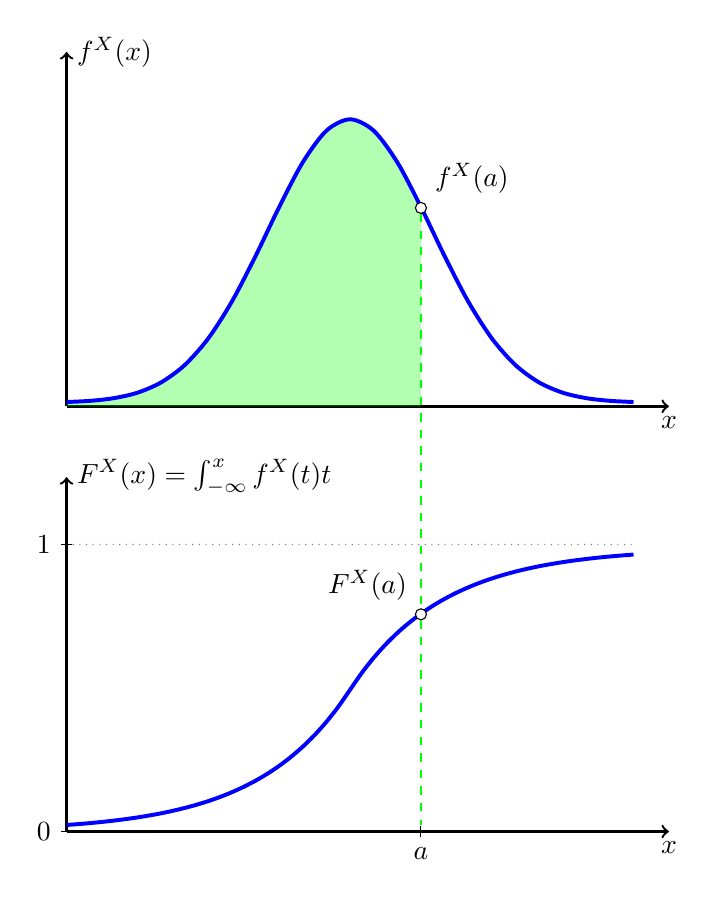
\begin{tikzpicture}[scale=0.9]
		\draw[->, line width=0.3mm] (0,6) to (8.5,6) node[below] {$x$};
		\draw[->, line width=0.3mm] (0,6) to (0,11) node[right] {$f^X(x)$};
		\draw[->, line width=0.3mm] (0,0) to (8.5,0) node[below] {$x$};
		\draw[->, line width=0.3mm] (0,0) to (0,5) node[right] {$F^X(x)=\int_{-\infty}^x f^X(t)\intd t$};

		\filldraw[line width=0.5mm,scale=1,domain=0:5,smooth,variable=\x, draw=none, fill=green, opacity=0.3] plot ({\x},{4*exp(-(\x-4)*(\x-4)/2.7)+6.05}) -- (5,6) -- (0,6);
		\draw[line width=0.5mm,scale=1,domain=0:8,smooth,variable=\x,blue] plot ({\x},{4*exp(-(\x-4)*(\x-4)/2.7)+6.05});


		\draw[line width=0.5mm,scale=1,domain=0:4,smooth,variable=\x,blue] plot ({\x},{2*exp((\x-4)/1.3)});
		\draw[line width=0.5mm,scale=1,domain=4:8,smooth,variable=\x,blue] plot ({\x},{-2*exp(-(\x-4)/1.3)+4});

		\draw (5,8.8) node (fa) [fill = white,circle,inner sep = 0pt,minimum size = 4pt,draw, label={above right:$f^X(a)$}] {};
		\draw (5,3.065) node (Fa) [fill = white,circle,inner sep = 0pt,minimum size = 4pt,draw, label={above left:$F^X(a)$}] {};
		\draw (5,0) node (a) [fill = white,rectangle,inner sep = 0pt,minimum size = 0pt,minimum height=4pt,draw, label={below:$a$}] {};
		%\draw (5,6) node (a2) [fill = white,rectangle,inner sep = 0pt,minimum size = 0pt,minimum height=4pt,draw, label={below right:$a$}] {};

		\draw[dashed, line width=0.3mm, green] (fa) -- (Fa) -- (a);

		\draw (0,0) node (null) [fill = white,rectangle,inner sep = 0pt,minimum size = 0pt,minimum width=4pt,draw, label={left:$0$}] {};
		\draw (0,4.05) node (eins) [fill = white,rectangle,inner sep = 0pt,minimum size = 0pt,minimum width=4pt,draw, label={left:$1$}] {};
		\draw[dotted, gray] (eins) -- (8, 4.05);
	\end{tikzpicture}	
\end{center}

\paragraph{Bemerkung:}
Aus der Normiertheit von $P$ folgt, dass
\begin{equation*}
	\int_{-\infty}^\infty f(t)\intd t=1
\end{equation*}

\begin{definition}{Erwartungswert und Varianz im allgemeinen W-Raum}
	Analog zur Definition von Erwartungswert und Varianz einer Zufallsvariablen sind die beiden Kennzahlen definiert als
	\begin{align*}
		E(X)&=\int_{-\infty}^\infty x*f(x)\intd x\\
		V(X)&=\int_{-\infty}^\infty (x-E(X))^2 * f(x)\intd x = E((X-E(X))^2) = \sigma(X)^2.
	\end{align*}
\end{definition}


\section{Stetige Verteilungen}